
\documentclass{beamer}
\usepackage[orientation=portrait, size=a1, scale=1.4, debug]{beamerposter}
\usetheme{unn}

\usepackage{cmbright}

\usepackage{fontspec}
\usepackage{indentfirst}


\setmainfont{Times New Roman}
\setromanfont{Times New Roman}
\setsansfont{Times New Roman}

\usepackage{polyglossia}
\setmainlanguage{russian}
\usepackage{csquotes}

\usepackage{booktabs}
\usepackage{ragged2e}

\usepackage[backend=biber,
            movenames=false,
            maxnames=4,
            style=gost-numeric,
            sorting=none,
            autolang=other]{biblatex}
						
%\newfontfamily\cyrillicfonttt{lmmonolt10-regular.otf}
%\newfontfamily\cyrillicfontsf{lmsans10-regular.otf}						
					
\addbibresource{bibliography.bib}

\DeclareMathOperator{\re}{\operatorname{Re}}

\title{Параллельный алгоритм липшицевой глобальной оптимизации с двойной оценкой константы Липшица }
\author{К.А. Баркалов \and  Д.А. Черных}
\institute{Нижегородский государственный университет им. Н.И. Лобачевского}
\setlength{\abovedisplayskip}{3pt}
\setlength{\belowdisplayskip}{3pt}

%\bibliographystyle{unsrt}

\begin{document}
\begin{frame}[t]
    \begin{columns}[t]
        \begin{column}[t]{0.465\paperwidth}
            \begin{block}{Постановка задачи}
            
            \leftskip=0.5cm \rightskip=0.5cm 
            \setlength{\parindent}{1.25cm} %
            Рассмотрим задачу глобальной оптимизации вида\\
             \(\phi(y^*) = min\{\phi(y), y\in D\}\), где \(D=\{y\in R^N:a_i\leqslant y_i\leqslant{b_i}, 1\leqslant{i}\leqslant{N}\}\). 
             
             Будем предполагать, что целевая функция задана как <<черный ящик>> и удовлетворяет условию Липшица с априори неизвестной константой \(L\) \cite{Kvasov2013}. 
          \end{block}
          
          \begin{block}{Редукция размерности с помощью кривых Пеано}
\leftskip=0.5cm \rightskip=0.5cm 
\setlength{\parindent}{1.25cm} %
В ННГУ им. Н.И. Лобачевского под руководством проф. Р.Г. Стронгина разработан эффективный подход к решению задач глобальной оптимизации \cite{Strongin2013}. В рамках данного подхода решение многомерной задачи сводится к решению эквивалентной ей одномерной задачи. Для этого используется редукция размерности с помощью кривой Пеано \(y(x)\), которая непрерывно и однозначно отображает отрезок вещественной оси \([0,1]\) на \(N\)-мерный куб \cite{Sergeyev2013}.

\leftskip=0.02cm 
\setlength{\parindent}{0.02cm}
 \begin{minipage}[t]{.98\textwidth}
              \begin{figure}
                  %\centering
                  \center{\includegraphics[width=1.000\textwidth]{images/pean_2 (1)_8.jpg}}
                  %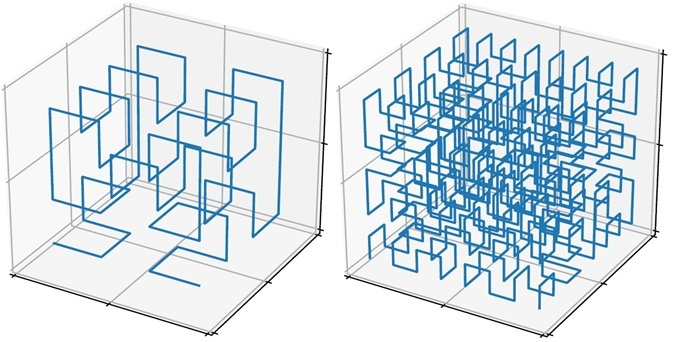
\includegraphics[scale=1.468]{images/pean_2.jpg}
                 % \caption{Построение кривой Пеано, заполняющей трехмерный куб}
              \end{figure}
              \end{minipage}
              


\end{block}
\begin{block}{Метод с  двойной оценкой константы Липшица}
\leftskip=0.5cm \rightskip=0.5cm 
\setlength{\parindent}{1.25cm} %
Алгоритм строит последовательность точек \(x^k\), в которых проводятся \textit{испытания}, т.е. вычисляются значения целевой функции \(\phi^k=\phi(y(x^k))\).

В исследуемом методе для достижения более точного значения константы \(L\) используются заниженная и завышенная оценки константы Липшица\cite{Strongin2020}. Большая оценка гарантирует глобальную сходимость алгоритма, меньшая снижает число поисковых испытаний, требующихся для поиска решения задачи.

Распараллеливание организовано следующим образом: в ходе выполнения одной итерации алгоритма одновременно проводятся \(P \geq 1\) испытаний в наиболее перспективных точках области поиска. В прикладных задачах глобальной оптимизации проведение даже одного испытания является трудоемкой операцией. Поэтому параллельное проведение нескольких испытаний повышает скорость работы алгоритма. 
\leftskip=0.001cm 
\setlength{\parindent}{0.001cm}
 \begin{minipage}[t]{0.96\textwidth}
              \begin{figure}
                 % \centering
                 \center{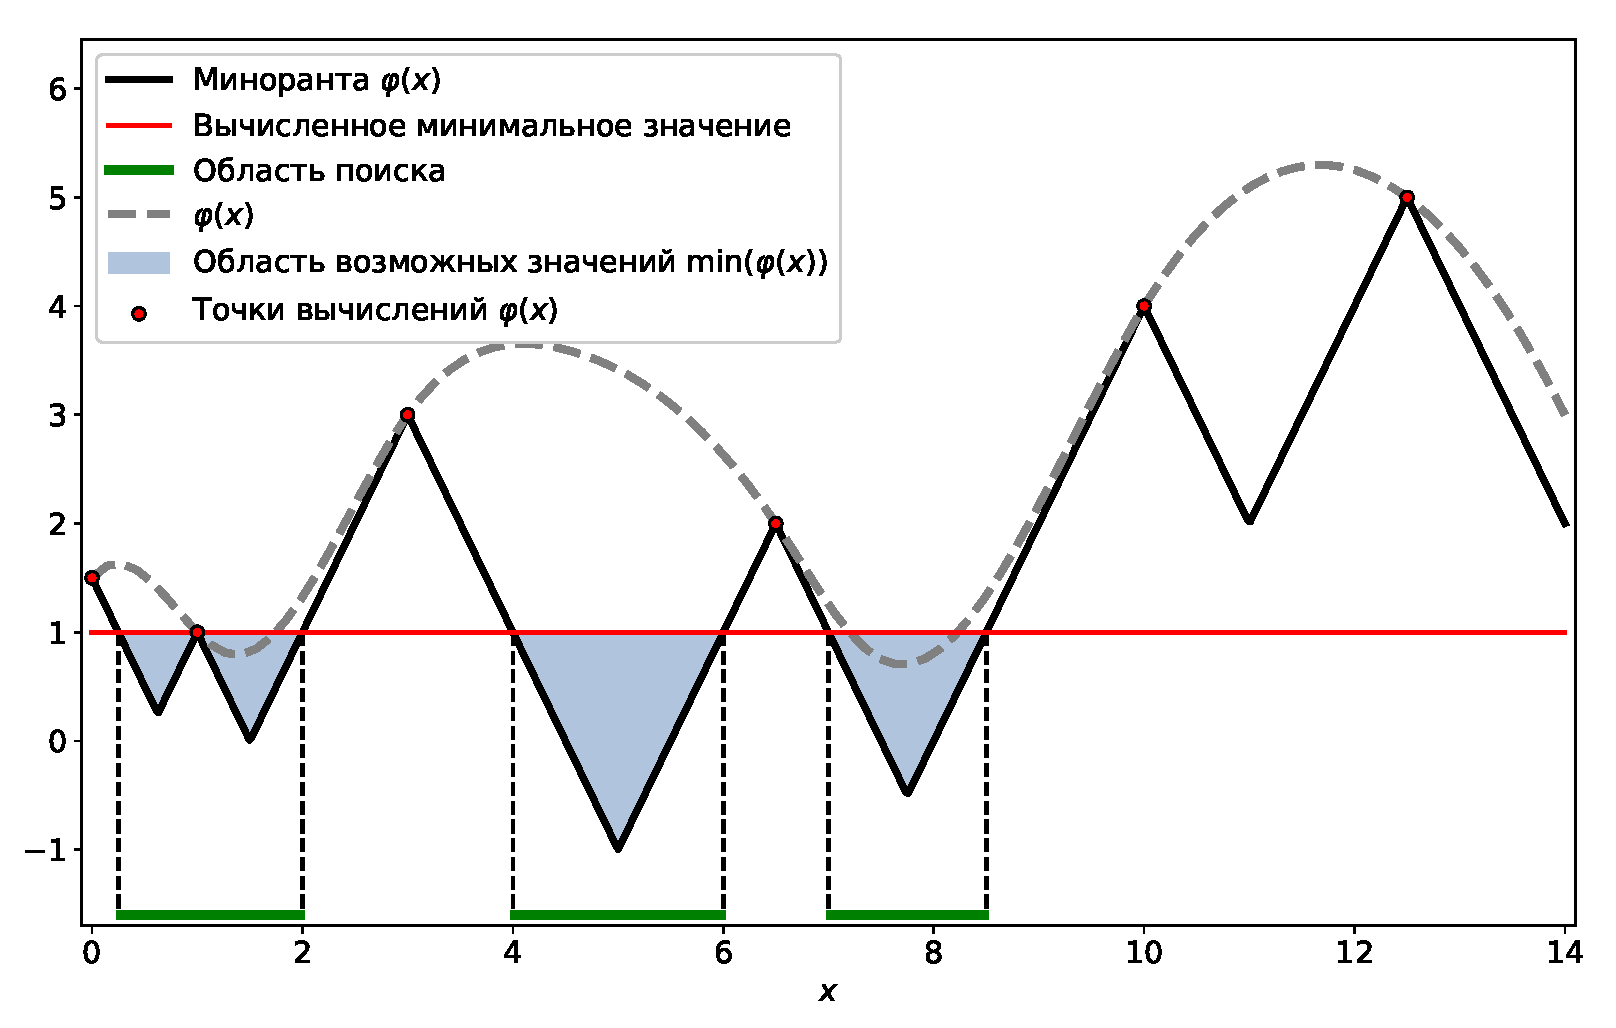
\includegraphics[width=1.045\textwidth]
                 {images/PGS2.eps}}
                % \includegraphics[scale=1.095]{images/PlotGS_7.png}
                %  \caption{}
              \end{figure}
              \end{minipage}
\end{block}
            
        \end{column}
        \begin{column}[t]{0.47\paperwidth}
          \begin{block}{Общая схема параллельного алгоритма}
\leftskip=0.5cm \rightskip=0.5cm 
\setlength{\parindent}{1.25cm} %
Одна итерация состоит в выполнении следующих действий:
              \begin{enumerate}
              \leftskip=0.5cm \rightskip=0.5cm 
\setlength{\parindent}{1.25cm} %
                \justifying
                \item Упорядочить точки предшествующих испытаний в порядке возрастания их координат: \(x_{0}<...<x_{i}<...<x_{k}\);
                \item Для каждого интервала \((x_{i-1}, x_{i}),1\leqslant i\leqslant k,\) вычислить две \textit{характеристики} \(R_{glob}(i), R_{loc}(i)\), отвечающие за завышенную и заниженную оценки константы Липшица;
                \item Вычислить характеристику \(R(i) = \max⁡\{\rho*R_{loc}(i),R_{glob}(i)\}\), где \(\rho\) -- весовой коэффициент; 
                % \(\rho=((1-1/r_{glob} )/(1-1/r_{loc} ))^2\)
                \item Упорядочить характеристики \(R(i)\) в порядке убывания \(R(t_{1})\geqslant R(t_{2})\geqslant ... \geqslant  R(t_{k-1})\geqslant R(t_{k})\) и выбрать \(P\) интервалов \((x_{t_j-1}, x_{t_j}), 1\leqslant j \leqslant P,\) с наибольшими характеристиками;
                \item Провести следующие испытания параллельно в точках  \(x^{k+j} \in (x_{t_j-1}, x_{t_j})\), \(1\leqslant j \leqslant P,\) вычисляемых согласно правилу размещения точки следующего испытания в интервале с заданным номером \(t_j\);
                \item Проверить выполнение критерия остановки \(\Delta_{t_j}<\varepsilon, 1\leqslant j \leqslant P\).
              \end{enumerate}

\end{block}

%----------------------------------------------------------------------------------------
%	RESULTS
%----------------------------------------------------------------------------------------

\begin{block}{Результаты экспериментов с использованием OpenMP}

\leftskip=0.5cm \rightskip=0.5cm 
\setlength{\parindent}{1.25cm} %
При реализации параллельного алгоритма использовалась технология \textit{OpenMP} для программирования многопоточных приложений на многопроцессорных системах с общей памятью.

Достоинствами \textit{OpenMP} являются простота, открытость, возможность легкой интеграции в существующий код, а так же возможность инкрементального программирования.
 
На данный момент получены результаты вычислительных экспериментов на тестовых задачах, формируемых специальным генератором \cite{GKLS}. В таблице \ref{table:GKLS_RES_1} приведены среднее число итераций параллельной реализации метода с двойной оценкой константы Липшица и ускорение относительно последовательной версии. В эксперименте решалось 100 задач размерности \(N = 2\). Результаты получены на узле суперкомпьютера <<Лобачевский>> (процессор AMD EPYC 7742 64-Core, 40 GB RAM, видеокарта NVIDIA GA100), использовался язык \textit{C++} с технологией \textit{OpenMP} .


%{\setlength{\extrarowheight}{5pt}

\begin{table}[!hbp]
    \centering
    \caption{Результаты решения серии задач размерности $N=2$}
     \renewcommand{\arraystretch}{1.4}
    \renewcommand{\tabcolsep}{1cm}
    \begin{tabular}{|c|c|c|c|}
    \hline
    P  & Итерации  & Время работы (сек.) & Ускорение \\ \hline
        16 & 15.2 & 6.52 & 10.87  \\ \hline
	32 & 8.12 & 3.75 & 18.9  \\ \hline
	64 & 5.04 & 3.00 & 23.62 \\ \hline
	\end{tabular}
    
    \label{table:GKLS_RES_1}
\end{table}

\end{block}
          \begin{block}{Литература}
            %\bibliographystyle{unsrt}
            %\bibliography{bibliography}
            \printbibliography

            
          \end{block}
        \end{column}
    \end{columns}
\end{frame}
\end{document}